\documentclass[tikz,border=3pt]{standalone}
\usepackage[T1]{fontenc}
\usepackage{newtxtext,newtxmath}
\usetikzlibrary{arrows.meta,positioning,fit,shapes.geometric}
\begin{document}
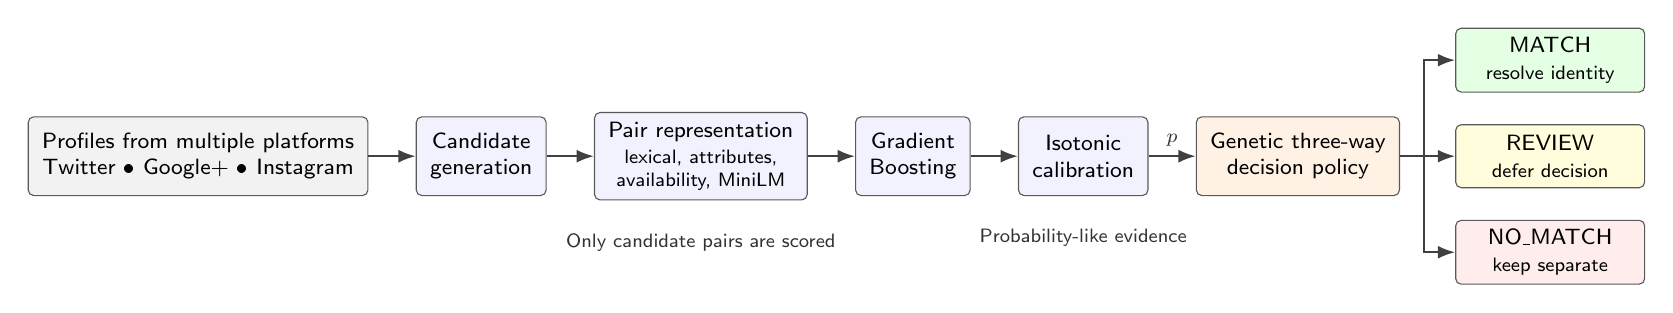
\begin{tikzpicture}[
  font=\sffamily\footnotesize,
  stage/.style={draw=black!65, rounded corners=2pt, fill=blue!5, minimum height=10mm, align=center, inner xsep=5pt},
  input/.style={stage, fill=gray!10},
  decision/.style={stage, fill=orange!10},
  outcome/.style={draw=black!65, rounded corners=2pt, minimum width=24mm, minimum height=8mm, align=center},
  arrow/.style={-{Latex[length=2.2mm]}, thick, draw=black!75},
  note/.style={font=\sffamily\scriptsize, align=center, text=black!80}
]
\node[input] (profiles) {Profiles from multiple platforms\\Twitter \textbullet\ Google+ \textbullet\ Instagram};
\node[stage, right=6mm of profiles] (block) {Candidate\\generation};
\node[stage, right=6mm of block] (features) {Pair representation\\\scriptsize lexical, attributes,\\[-1pt]\scriptsize availability, MiniLM};
\node[stage, right=6mm of features] (gb) {Gradient\\Boosting};
\node[stage, right=6mm of gb] (cal) {Isotonic\\calibration};
\node[decision, right=6mm of cal] (policy) {Genetic three-way\\decision policy};
\draw[arrow] (profiles)--(block);
\draw[arrow] (block)--(features);
\draw[arrow] (features)--(gb);
\draw[arrow] (gb)--(cal);
\draw[arrow] (cal)--node[note,above]{$p$}(policy);
\node[outcome, fill=green!10, above right=3mm and 7mm of policy] (match) {MATCH\\\scriptsize resolve identity};
\node[outcome, fill=yellow!14, right=7mm of policy] (review) {REVIEW\\\scriptsize defer decision};
\node[outcome, fill=red!7, below right=3mm and 7mm of policy] (nomatch) {NO\_MATCH\\\scriptsize keep separate};
\draw[arrow] (policy.east) -- ++(3mm,0) |- (match.west);
\draw[arrow] (policy.east) -- (review.west);
\draw[arrow] (policy.east) -- ++(3mm,0) |- (nomatch.west);
\node[note, below=3mm of features] {Only candidate pairs are scored};
\node[note, below=3mm of cal] {Probability-like evidence};
\end{tikzpicture}
\end{document}
